% ════════════════════════════════════════════════════════════════
%  CHAPITRE 4 — CONCEPTION ET RÉALISATION
% ════════════════════════════════════════════════════════════════

\chapter{Conception et réalisation}
\graphicspath{{Isipfe/Figures/}{diagramms/}}

% ── Introduction du chapitre ────────────────────────────────────
\section*{Introduction}
\addcontentsline{toc}{section}{Introduction}

Ce chapitre présente la conception et la réalisation de la solution selon
une organisation en releases Scrum, avec objectifs, conception,
implémentation et résultat observable côté utilisateur.

\textbf{Organisation en releases (Scrum) :}
\begin{itemize}
    \item \textbf{Release 1} : flux métier principal (authentification,
    candidature, pipeline RH) ;
    \item \textbf{Release 2} : enrichissement fonctionnel (analyse,
    planification, notifications) ;
    \item \textbf{Release 3} : consolidation (sécurité, gouvernance,
    robustesse opérationnelle).
\end{itemize}

Chaque release se termine par un incrément exploitable. La release
suivante enrichit ce socle sans remettre en cause les éléments déjà
validés, ce qui renforce la stabilité globale du produit.

\begin{figure}[H]
\centering
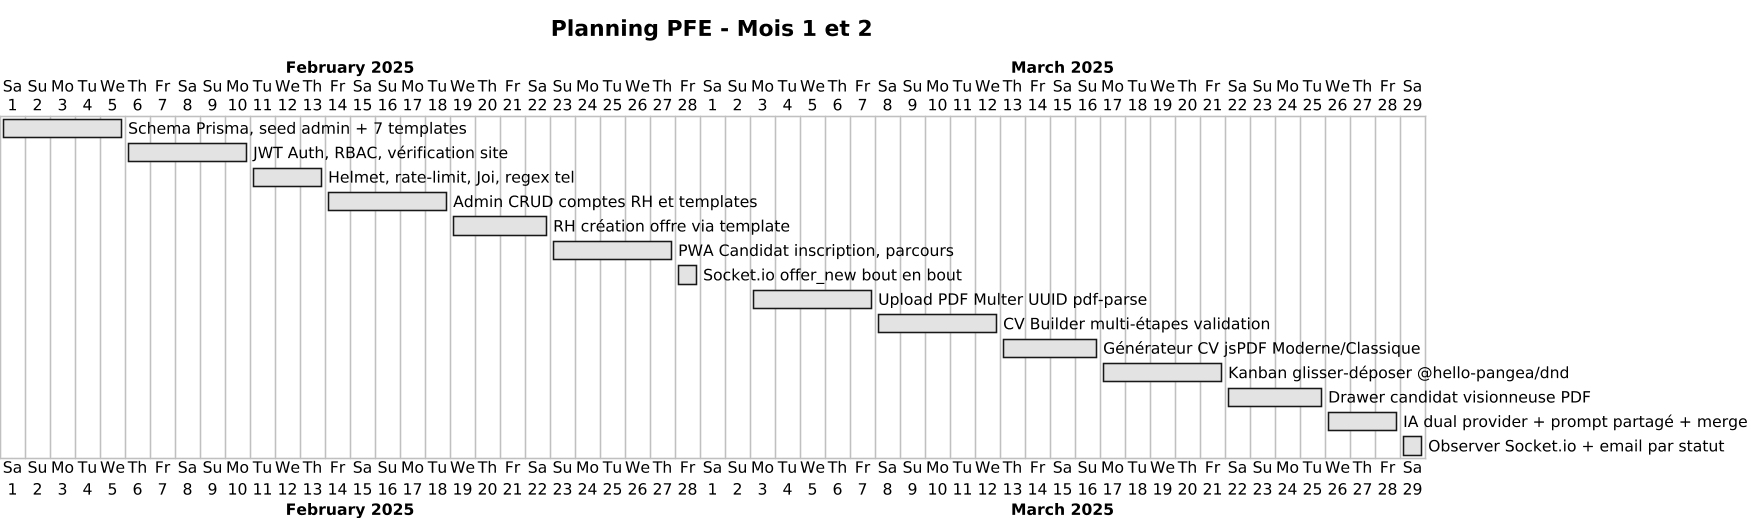
\includegraphics[width=0.85\textwidth]{gantt_mois_1_2}
\caption{Planification Scrum --- première phase}
\end{figure}

\begin{figure}[H]
\centering
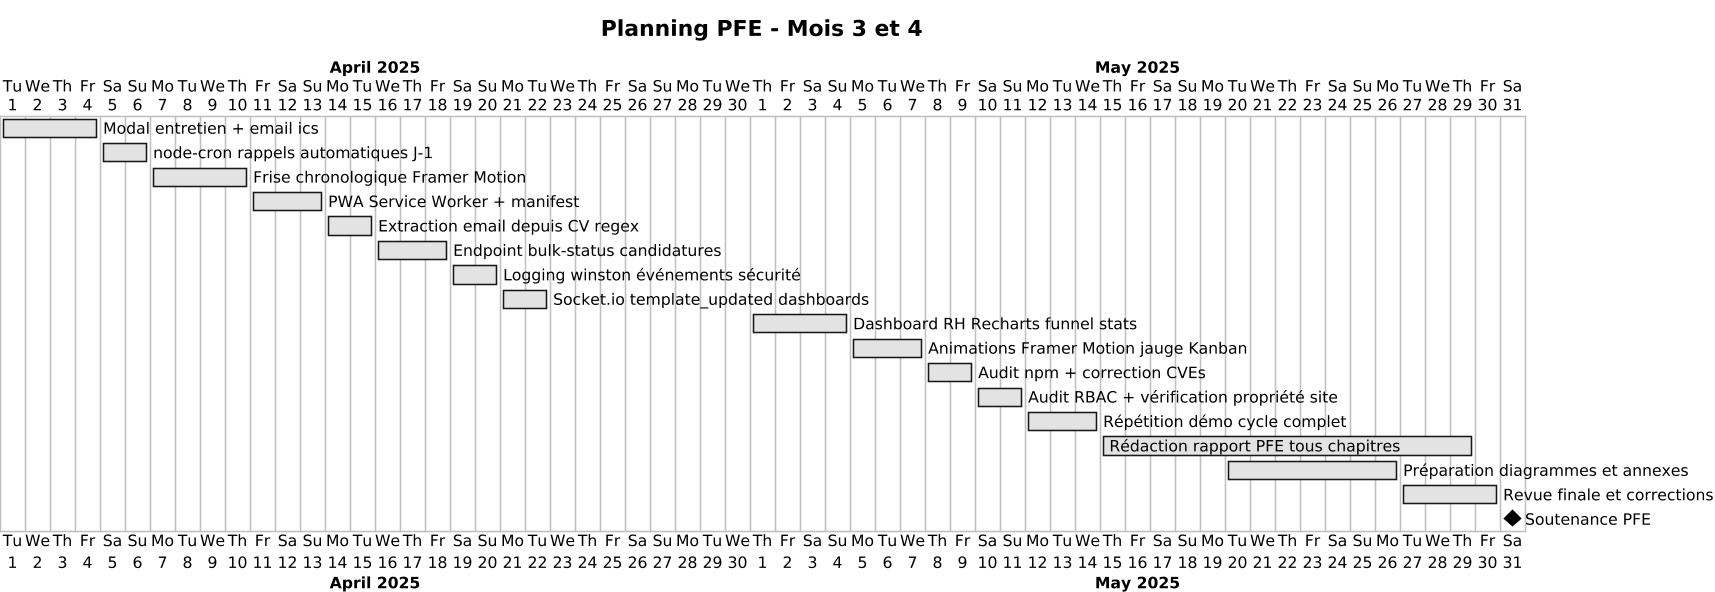
\includegraphics[width=0.85\textwidth]{gantt_mois_3_4}
\caption{Planification Scrum --- seconde phase}
\end{figure}

% ════════════════════════════════════════════════════════════════
\section{Release 1}
% ════════════════════════════════════════════════════════════════

\subsection{Objectifs}

La première release a pour objectif de livrer un flux complet et
directement utilisable :
création de compte candidat, consultation des offres, soumission de
candidature et traitement initial côté RH.

\subsection{User stories}

\begin{table}[H]
\centering
\caption{User stories principales de la Release 1}
\begin{tabularx}{\textwidth}{|l|X|l|}
\hline
\textbf{ID} & \textbf{User story} & \textbf{Priorité} \\
\hline
US1 & En tant que candidat, je crée un compte et je vérifie mon email. & Haute \\
\hline
US2 & En tant que candidat, je consulte les offres et je postule avec un CV. & Haute \\
\hline
US3 & En tant que RH, je visualise les candidatures reçues par site. & Haute \\
\hline
US4 & En tant que RH, je change l'état d'une candidature dans le pipeline. & Haute \\
\hline
US5 & En tant que candidat, je suis l'évolution de mon dossier. & Moyenne \\
\hline
\end{tabularx}
\end{table}

\subsection{Conception UML}

\subsubsection{Cas d'utilisation détaillés}

Nous avons d'abord validé les cas d'utilisation des deux acteurs
principaux de cette release (candidat et RH), afin de figer le périmètre
fonctionnel avant l'implémentation.

\begin{figure}[H]
\centering
\includegraphics[width=0.90\textwidth]{Cas_d’utilisation_détaillés_acteur_candidat}
\caption{Cas d'utilisation détaillés --- acteur candidat}
\end{figure}

\begin{figure}[H]
\centering
\includegraphics[width=0.90\textwidth]{Cas_d’utilisation_détaillés_Responsable_RH}
\caption{Cas d'utilisation détaillés --- acteur RH}
\end{figure}

\subsubsection{Diagrammes de séquence}

L'ordre de lecture des séquences suit le parcours réel d'un candidat :
inscription, vérification, connexion, puis candidature.

\begin{figure}[H]
\centering
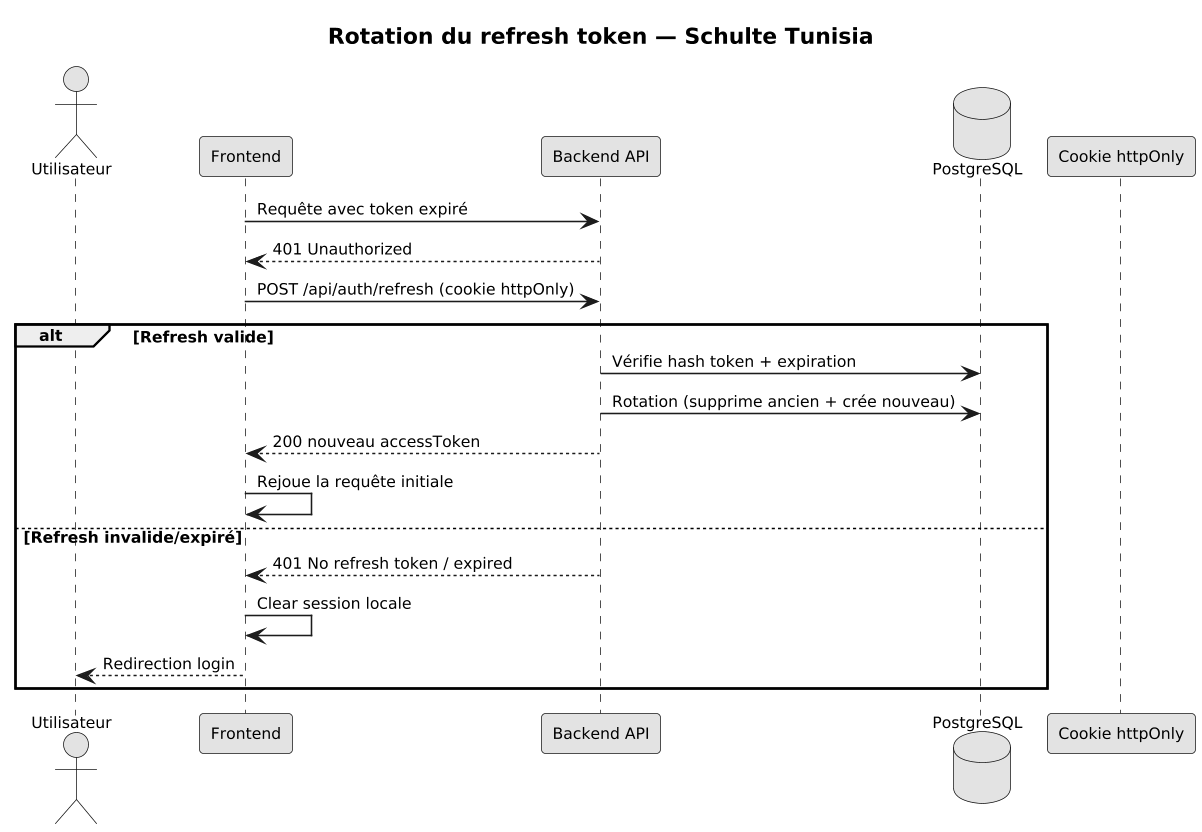
\includegraphics[width=0.90\textwidth]{inscription_candidat}
\caption{Séquence d'inscription du candidat}
\end{figure}

\begin{figure}[H]
\centering
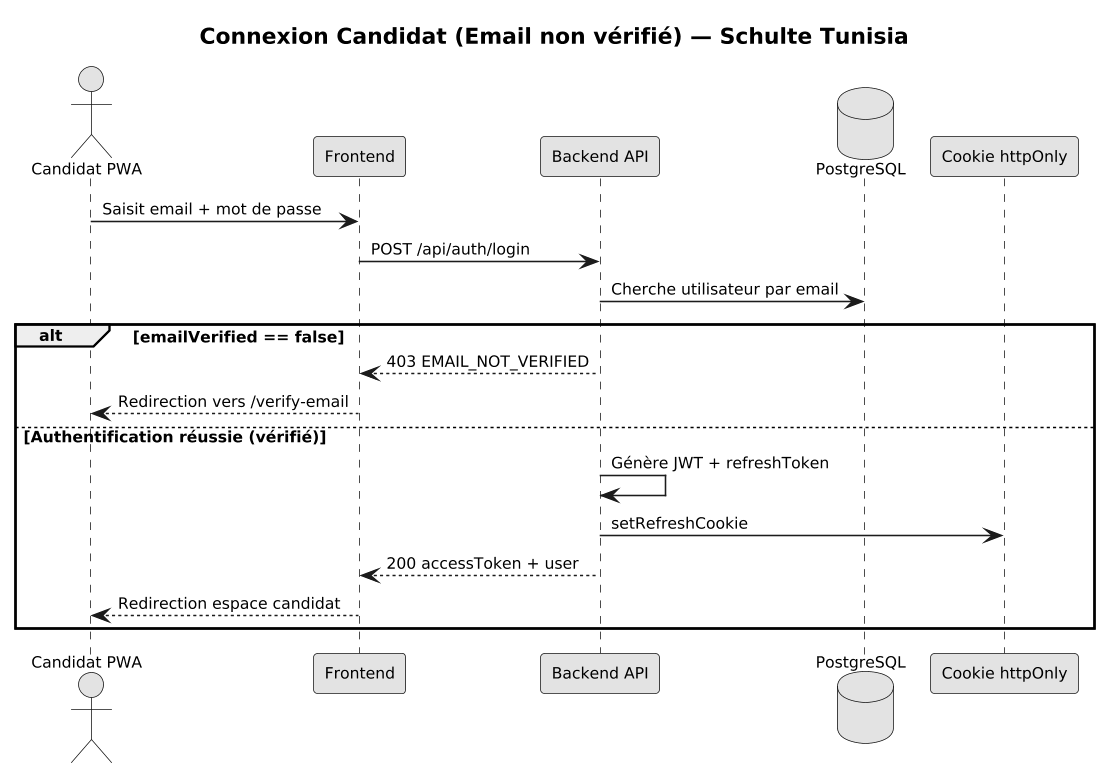
\includegraphics[width=0.90\textwidth]{tentative_connexion_avant_verification}
\caption{Blocage de connexion avant vérification email}
\end{figure}

\begin{figure}[H]
\centering
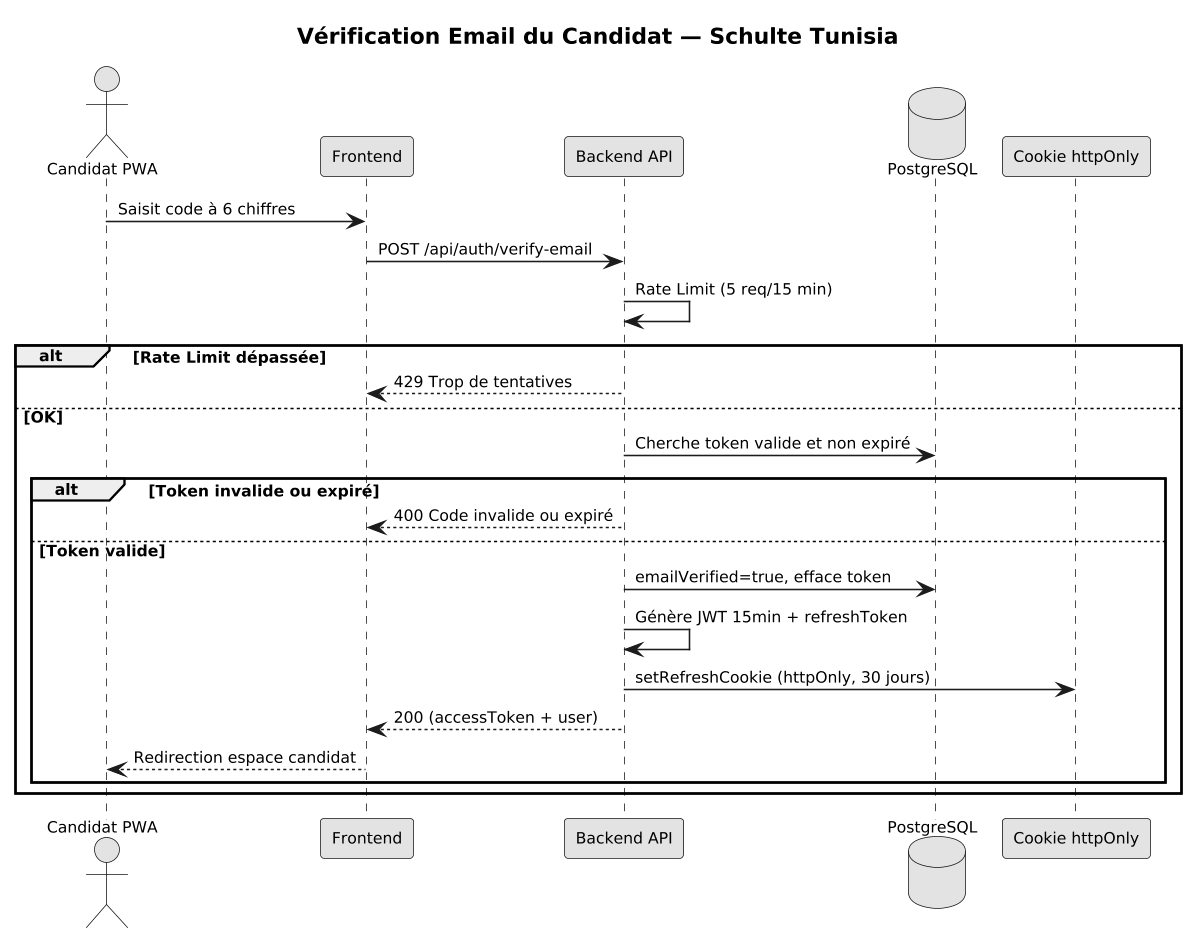
\includegraphics[width=0.90\textwidth]{verification_email_premiere_connexion}
\caption{Vérification email et première connexion}
\end{figure}

\begin{figure}[H]
\centering
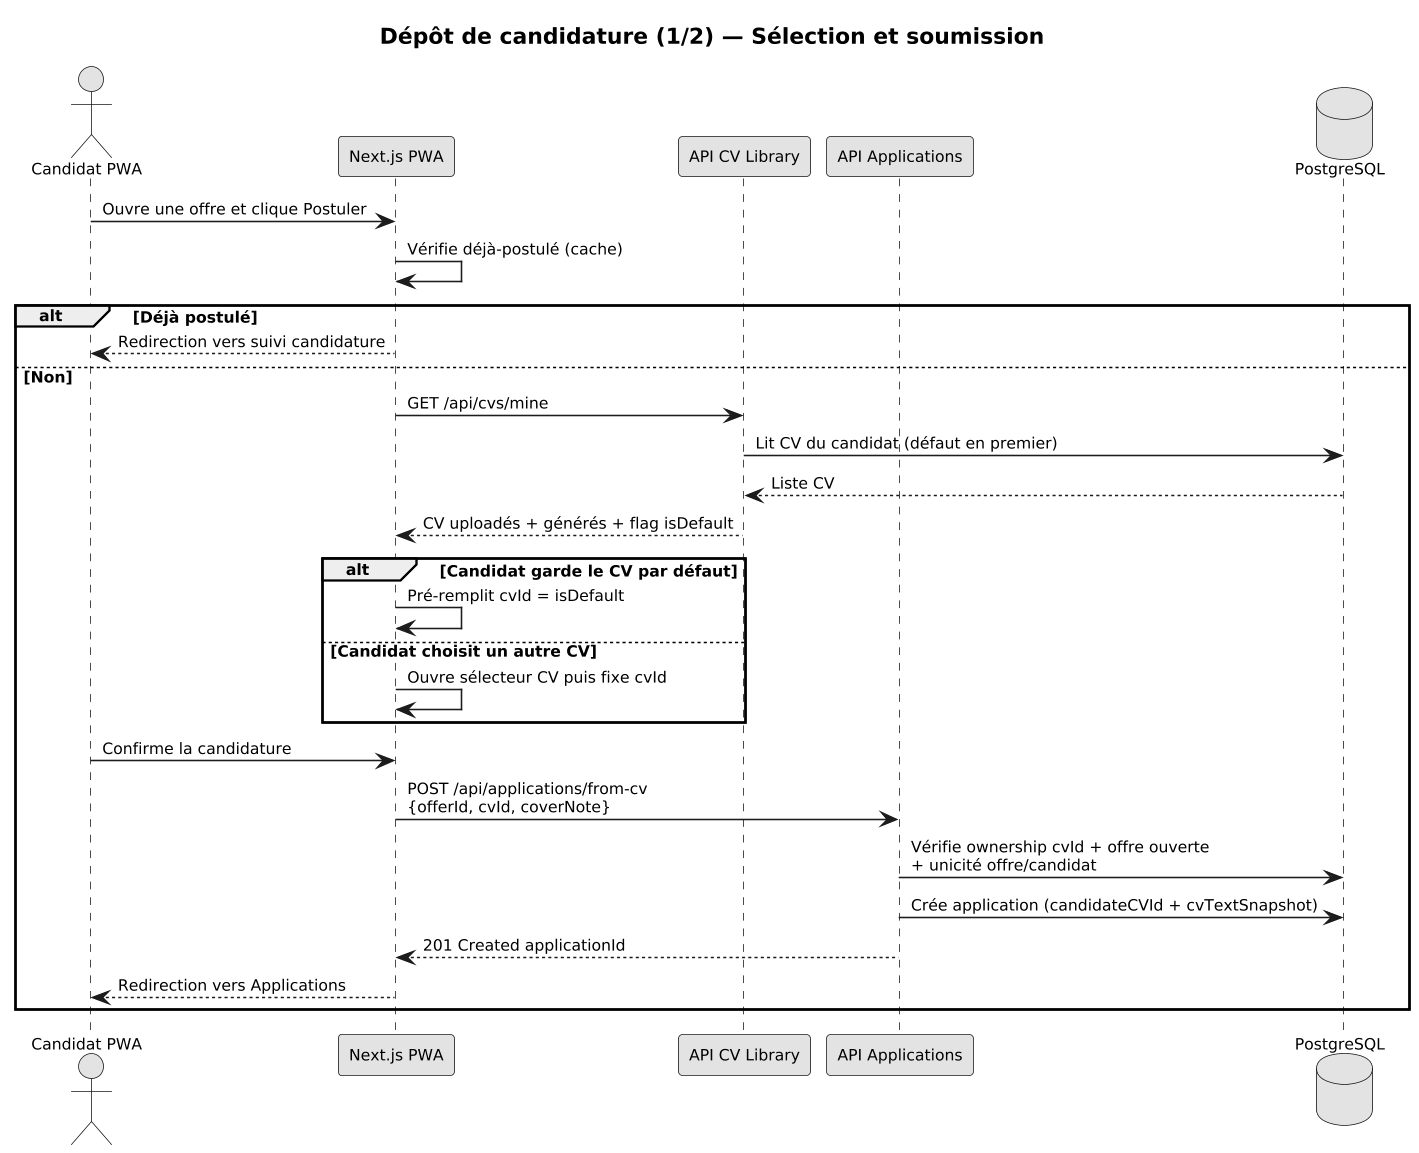
\includegraphics[width=0.90\textwidth]{selection_cv_soumission_candidature}
\caption{Séquence de sélection CV et soumission de candidature}
\end{figure}

\subsubsection{Diagrammes d'activité}

Après la soumission, le flux se poursuit côté RH. Les activités suivantes
représentent le traitement de la candidature dans le pipeline.

\begin{figure}[H]
\centering
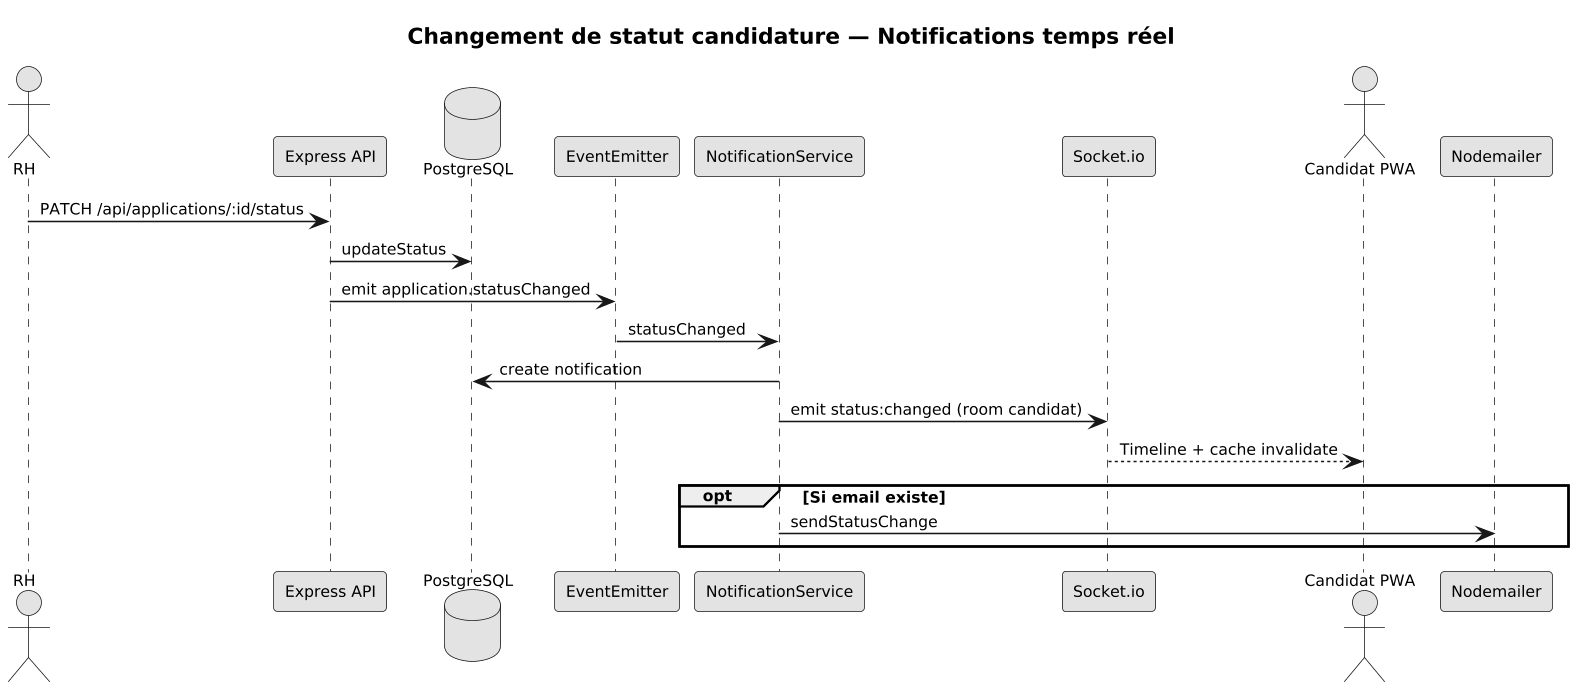
\includegraphics[width=0.90\textwidth]{changement_statut_candidature}
\caption{Activité de changement de statut d'une candidature}
\end{figure}

\begin{figure}[H]
\centering
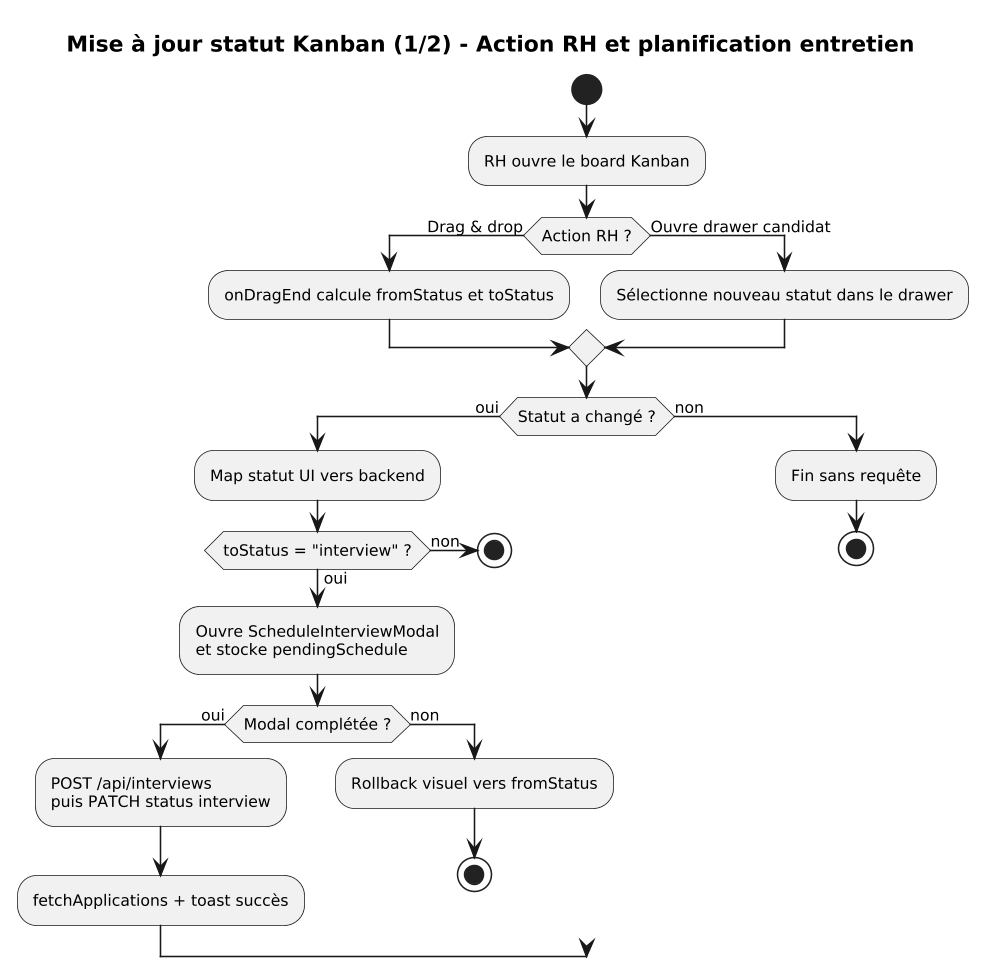
\includegraphics[width=0.90\textwidth]{action_rh_planification_statut_interview}
\caption{Activité RH de transition vers l'entretien}
\end{figure}

\subsubsection{Diagramme de classes}

Le modèle de classes métier a servi de base pour la persistance et les
relations entre candidats, offres, candidatures et entretiens.

\begin{figure}[H]
\centering
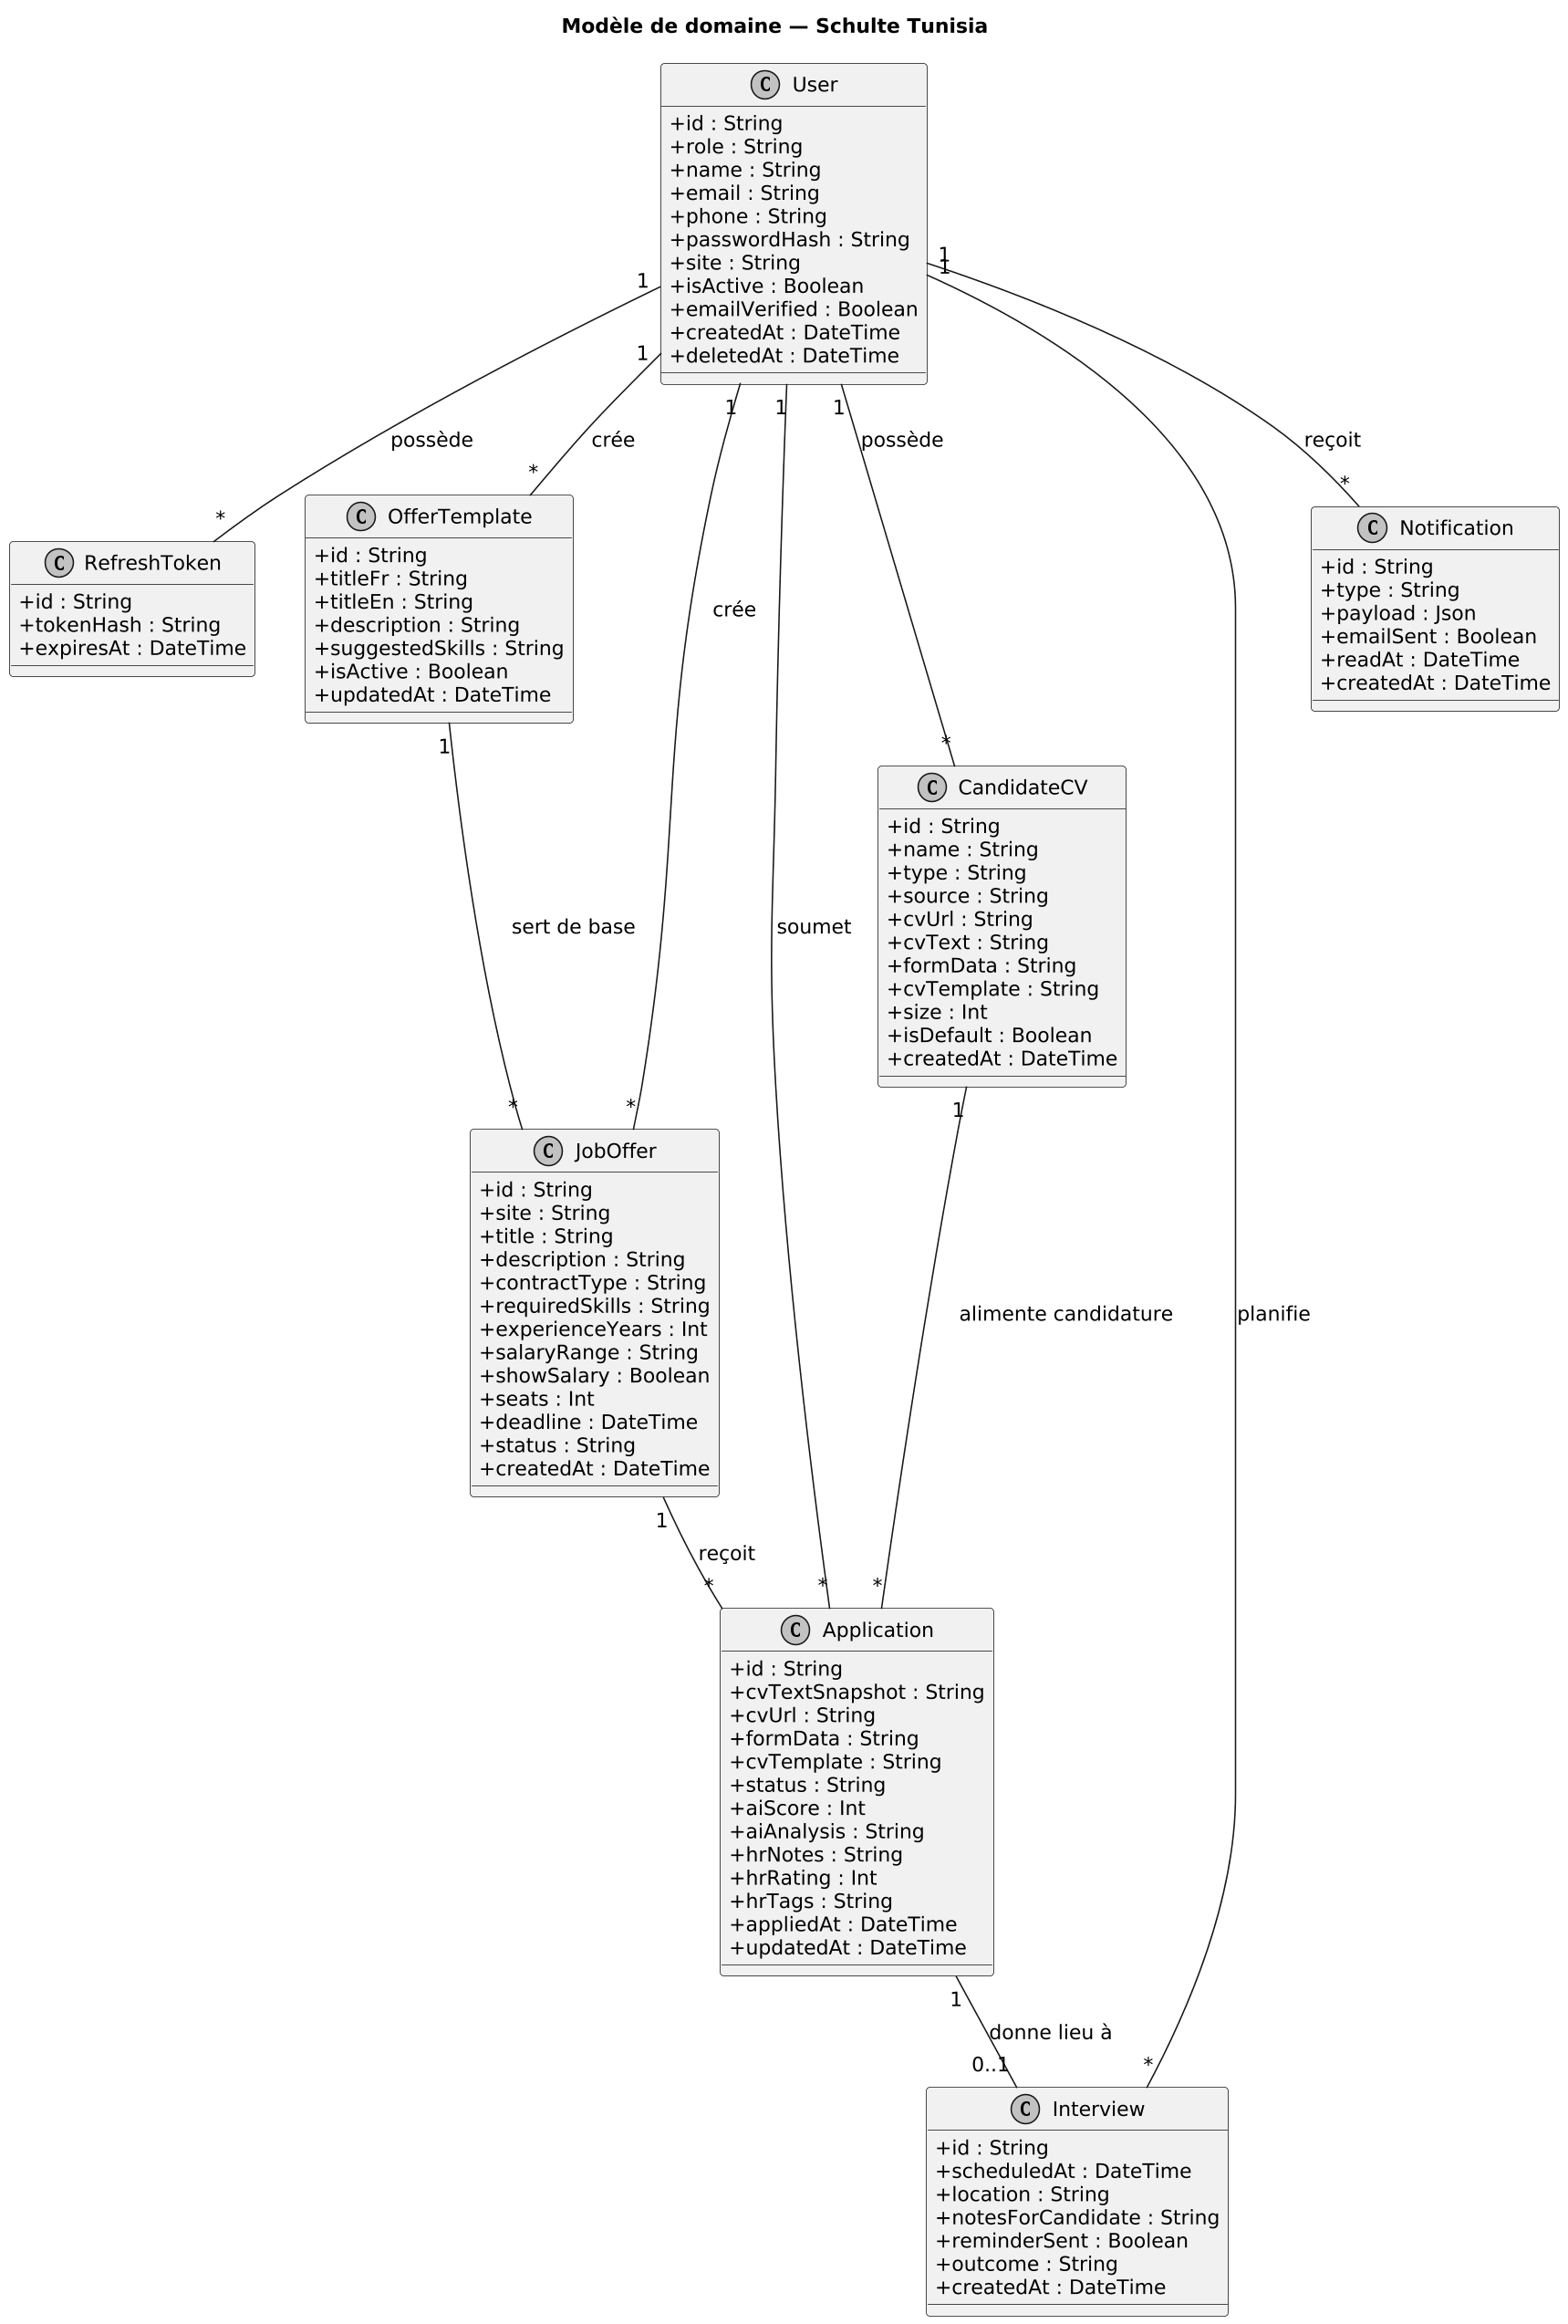
\includegraphics[width=0.90\textwidth]{diagramme_entites_metier}
\caption{Diagramme de classes métier de la plateforme}
\end{figure}

\subsection{Implémentation}

Cette release a été implémentée autour d'une API REST (Node.js/Express),
d'une base PostgreSQL (Prisma) et de deux interfaces clientes (PWA
candidat et interface RH). Les règles critiques appliquées dès cette phase
sont : contrôle par rôle, isolation par site, et workflow de statut.

Cette base confirme que la réalisation dépasse un CRUD classique : chaque
action applicative est contrainte par des règles métier explicites et des
conditions d'accès vérifiables.

\subsection{Interfaces}

Les interfaces réalisées dans cette release couvrent :
\begin{itemize}
    \item l'inscription/connexion candidat ;
    \item la consultation des offres et la soumission de candidature ;
    \item le tableau RH de suivi des candidatures.
\end{itemize}

Les captures suivantes illustrent le flux principal de bout en bout,
du point de vue candidat puis RH.

\begin{figure}[H]
\centering
\includegraphics[width=0.80\textwidth]{pwa_inscription.jpg}
\caption{Inscription candidat : point d'entrée du parcours}
\end{figure}

\begin{figure}[H]
\centering
\includegraphics[width=0.80\textwidth]{pwa_liste_offres.jpg}
\caption{Liste des offres disponibles sur la PWA}
\end{figure}

\begin{figure}[H]
\centering
\includegraphics[width=0.80\textwidth]{pwa_cv.jpg}
\caption{Gestion du CV avant la candidature}
\end{figure}

\begin{figure}[H]
\centering
\includegraphics[width=0.90\textwidth]{rh_kanban.jpg}
\caption{Pipeline RH (Kanban) pour le suivi des candidatures}
\end{figure}

% ════════════════════════════════════════════════════════════════
\section{Release 2}
% ════════════════════════════════════════════════════════════════

\subsection{Objectifs}

La deuxième release vise à améliorer la qualité de traitement RH et la
visibilité du processus pour le candidat, sans casser le flux métier
construit dans la release 1.

\subsection{Améliorations}

Les améliorations principales sont :
\begin{itemize}
    \item analyse assistée des candidatures ;
    \item planification des entretiens ;
    \item notifications et rappels ;
    \item meilleure lecture des dossiers côté RH.
\end{itemize}

\subsection{Conception}

La logique de conception de cette release repose sur un découplage clair :
les actions utilisateur restent rapides, tandis que les traitements lourds
(analyse, notifications) s'exécutent en asynchrone.

Cette organisation réduit les blocages côté interface, tout en conservant
la cohérence de l'état métier grâce à une persistance centrale et des
notifications synchronisées.

Les diagrammes suivants sont ordonnés selon le pipeline réel de la release :
analyse, consolidation des résultats, planification d'entretien, puis
notifications de suivi.

\begin{figure}[H]
\centering
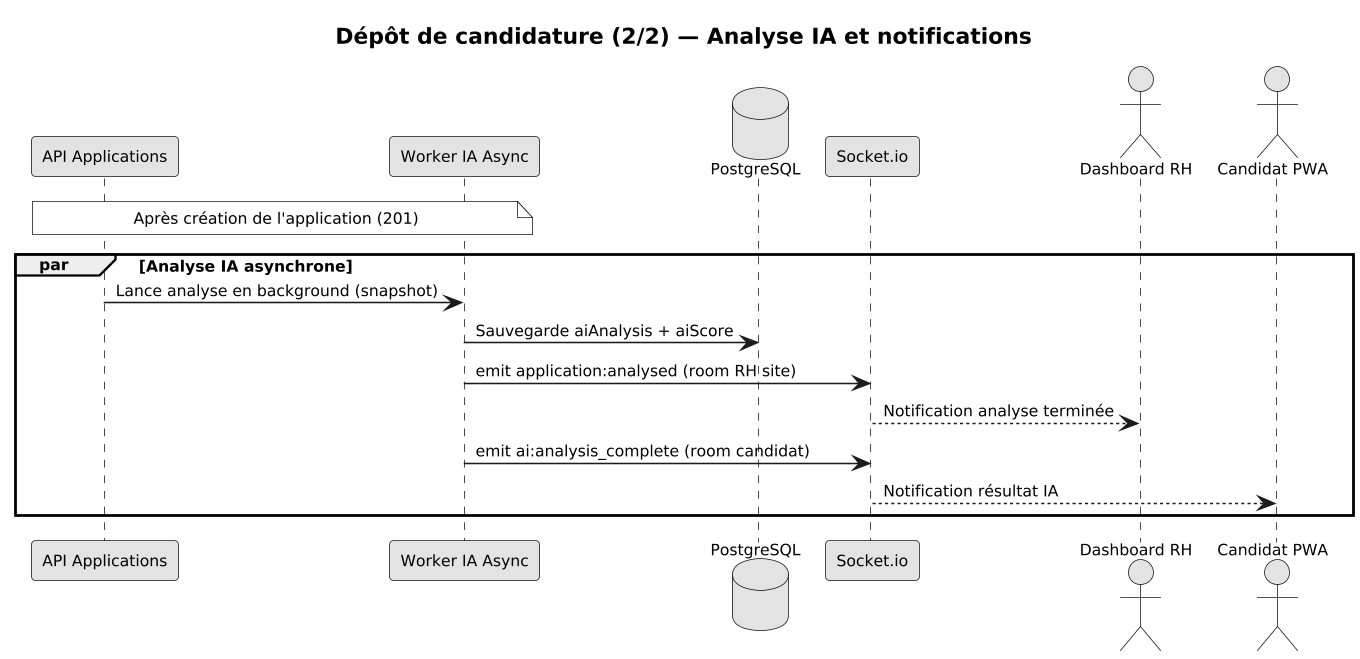
\includegraphics[width=0.90\textwidth]{analyse_ia_async_notifications_socket}
\caption{Conception asynchrone : analyse et notifications}
\end{figure}

\begin{figure}[H]
\centering
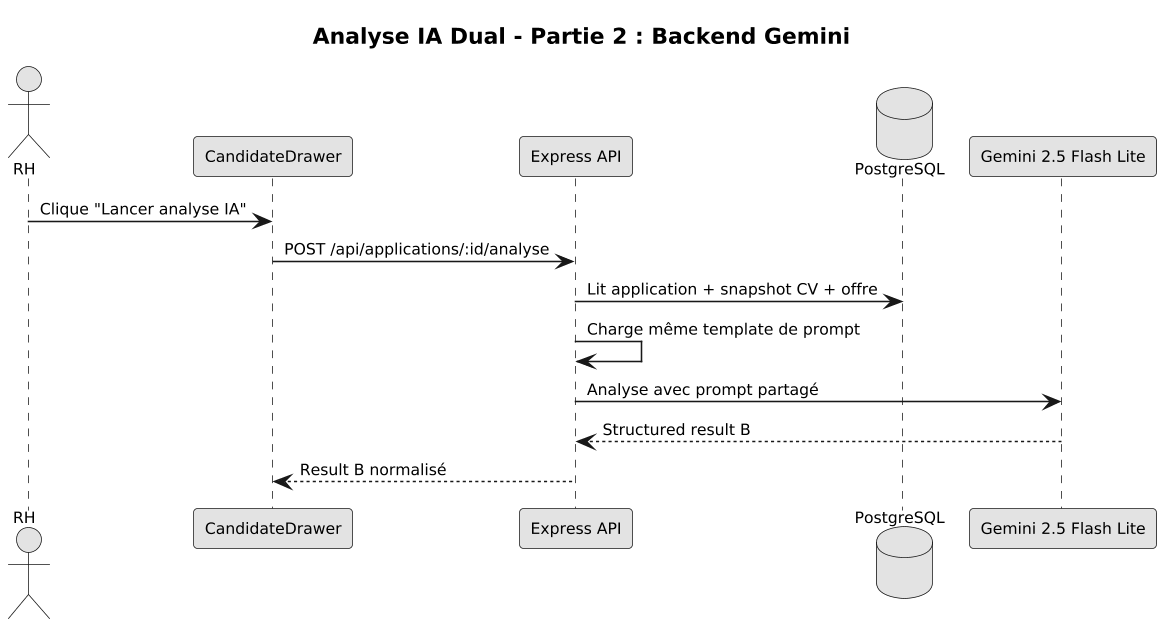
\includegraphics[width=0.90\textwidth]{analyse_backend_gemini}
\caption{Analyse côté backend (pipeline Gemini)}
\end{figure}

\begin{figure}[H]
\centering
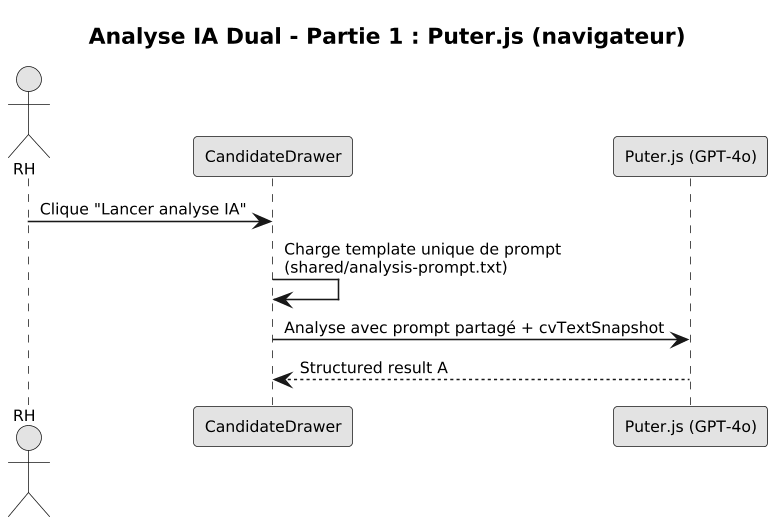
\includegraphics[width=0.90\textwidth]{analyse_puterjs}
\caption{Analyse complémentaire côté interface RH}
\end{figure}

\begin{figure}[H]
\centering
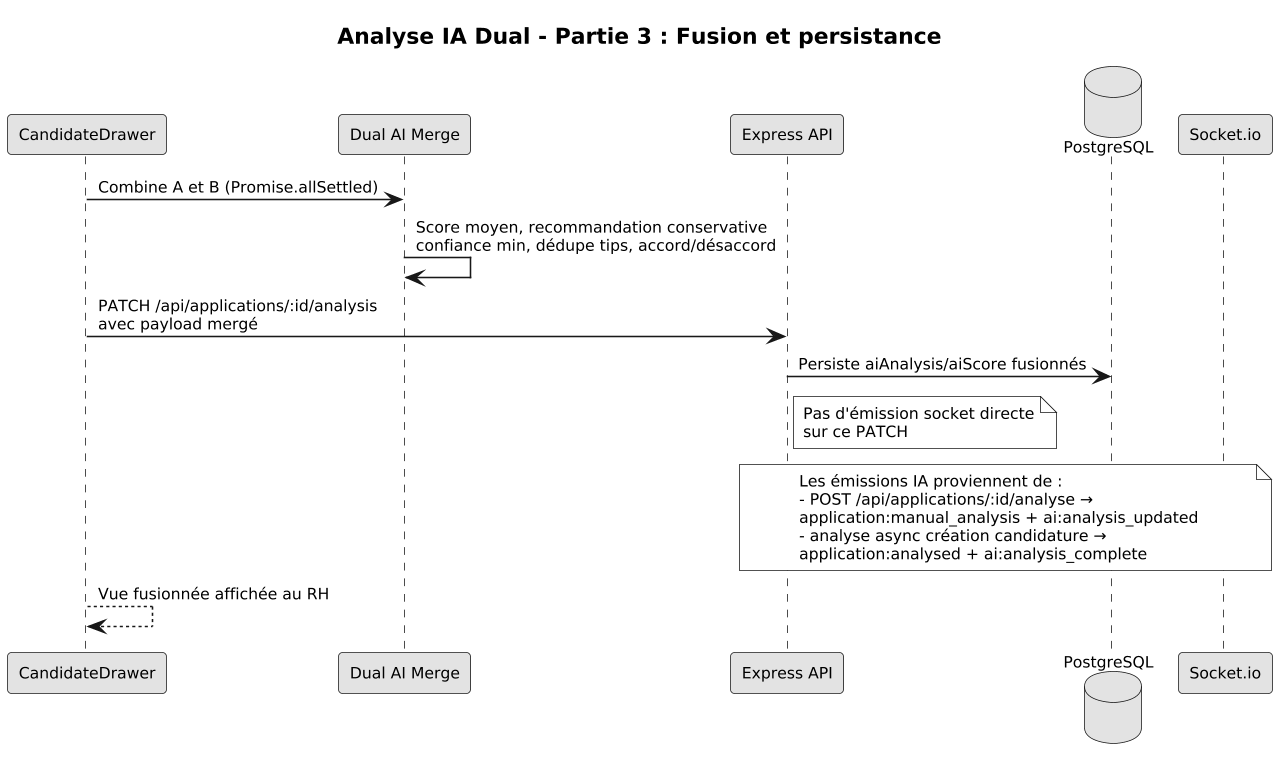
\includegraphics[width=0.90\textwidth]{fusion_resultats_persistance}
\caption{Fusion des résultats et persistance en base}
\end{figure}

\begin{figure}[H]
\centering
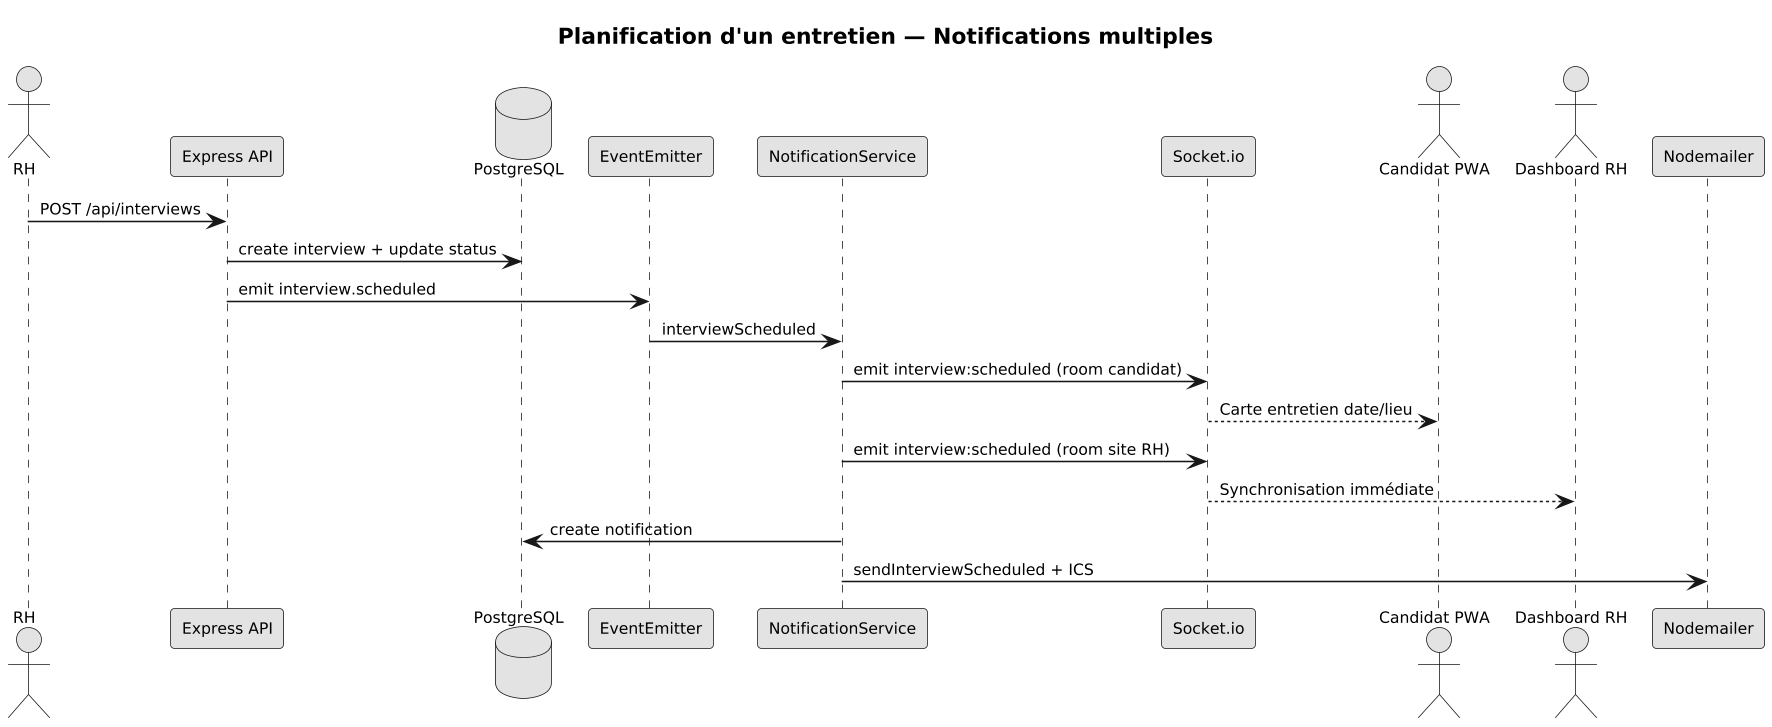
\includegraphics[width=0.90\textwidth]{planification_entretien_initiale}
\caption{Conception de la planification d'entretien}
\end{figure}

\begin{figure}[H]
\centering
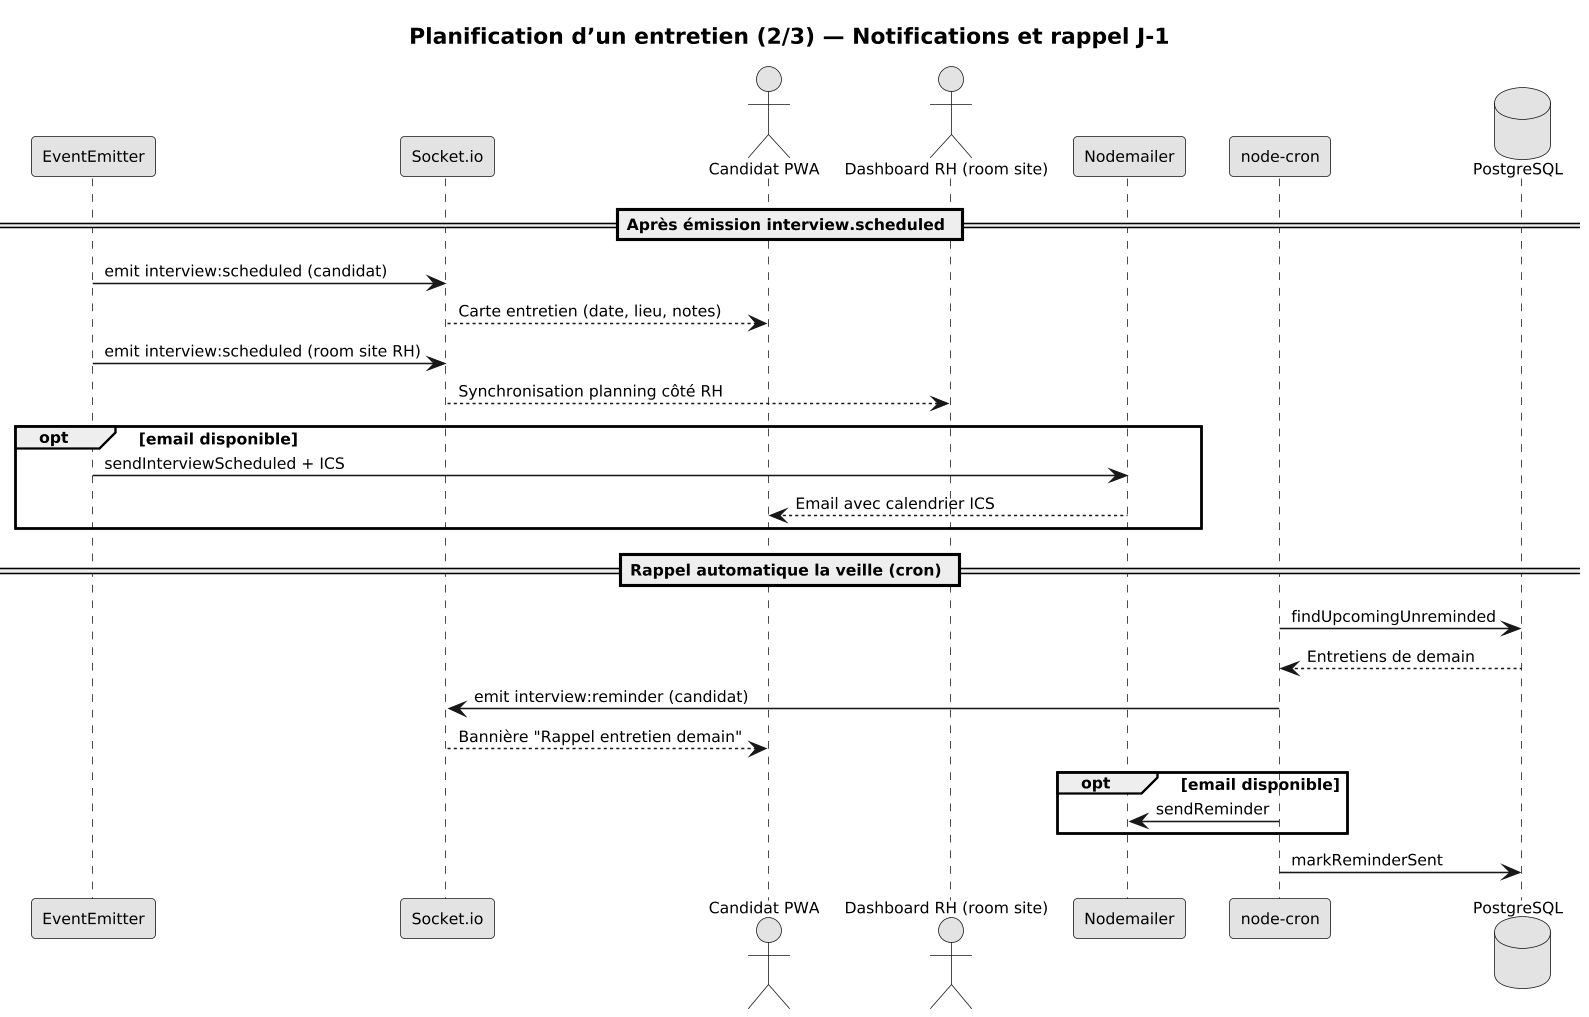
\includegraphics[width=0.90\textwidth]{notifications_rappel_automatique}
\caption{Conception des notifications et rappels automatiques}
\end{figure}

\subsection{Interfaces}

Les interfaces enrichies dans cette release sont :
\begin{itemize}
    \item le panneau RH de révision détaillée des candidatures ;
    \item les écrans de planification et suivi d'entretien ;
    \item le suivi candidat avec notifications plus explicites.
\end{itemize}

Ces écrans mettent en avant l'analyse, la décision RH et la visibilité
du processus côté candidat.

\begin{figure}[H]
\centering
\includegraphics[width=0.90\textwidth]{rh_panneau_candidat.jpg}
\caption{Panneau RH détaillé : décision et entretien}
\end{figure}

\begin{figure}[H]
\centering
\includegraphics[width=0.80\textwidth]{pwa_suivi_candidature.jpg}
\caption{Suivi de l'état de candidature côté candidat}
\end{figure}

\begin{figure}[H]
\centering
\includegraphics[width=0.80\textwidth]{pwa_notification.jpg}
\caption{Notifications et rappels visibles sur la PWA}
\end{figure}

% ════════════════════════════════════════════════════════════════
\section{Release 3}
% ════════════════════════════════════════════════════════════════

\subsection{Objectifs}

La troisième release vise la stabilisation de la solution pour un usage
fiable en conditions réelles :
sécurité, gouvernance des comptes et robustesse opérationnelle.

\subsection{Fonctionnalités (authentification, gestion utilisateurs)}

Les fonctionnalités ciblées sont :
\begin{itemize}
    \item renforcement de l'authentification et du cycle des sessions ;
    \item gestion complète des comptes RH par l'administrateur ;
    \item contrôle strict des accès API et WebSocket ;
    \item gestion du cycle de vie des comptes (activation/désactivation).
\end{itemize}

\subsection{Conception}

La conception suit une défense en profondeur : jetons, rotation,
révocation, contrôle par rôle et contrôle par site.

La séquence de lecture des diagrammes est volontaire : génération des
jetons, rotation, révocation/contrôle d'accès, puis gouvernance des
comptes RH.

\begin{figure}[H]
\centering
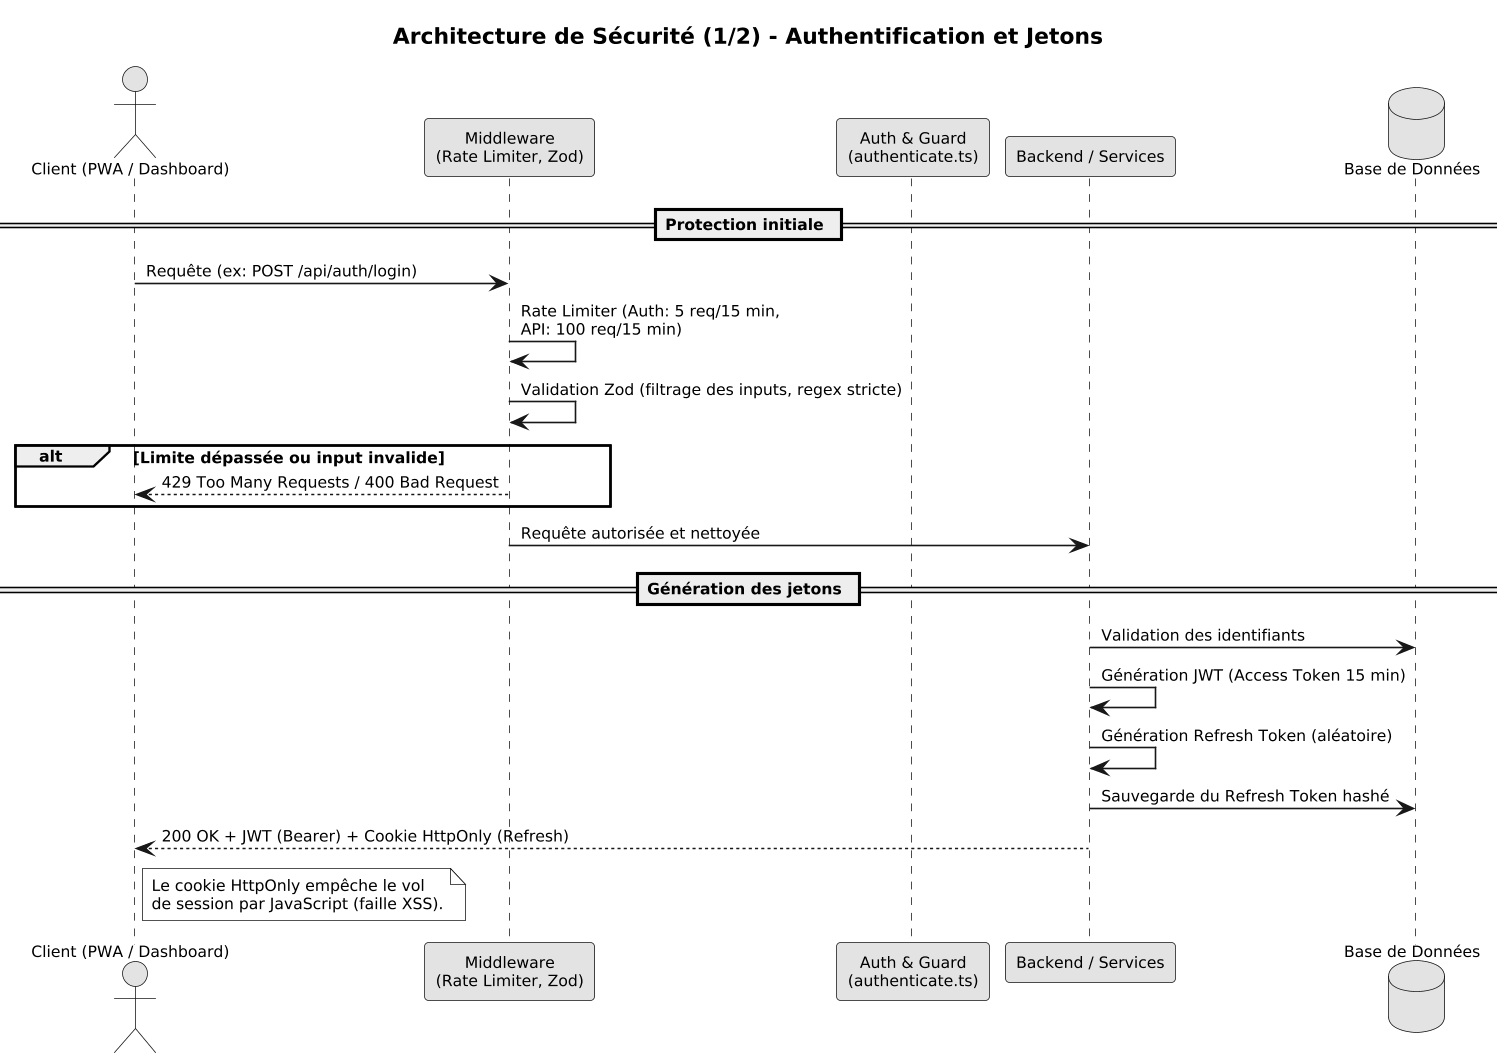
\includegraphics[width=0.90\textwidth]{authentification_generation_jetons}
\caption{Conception de l'authentification par jetons}
\end{figure}

\begin{figure}[H]
\centering
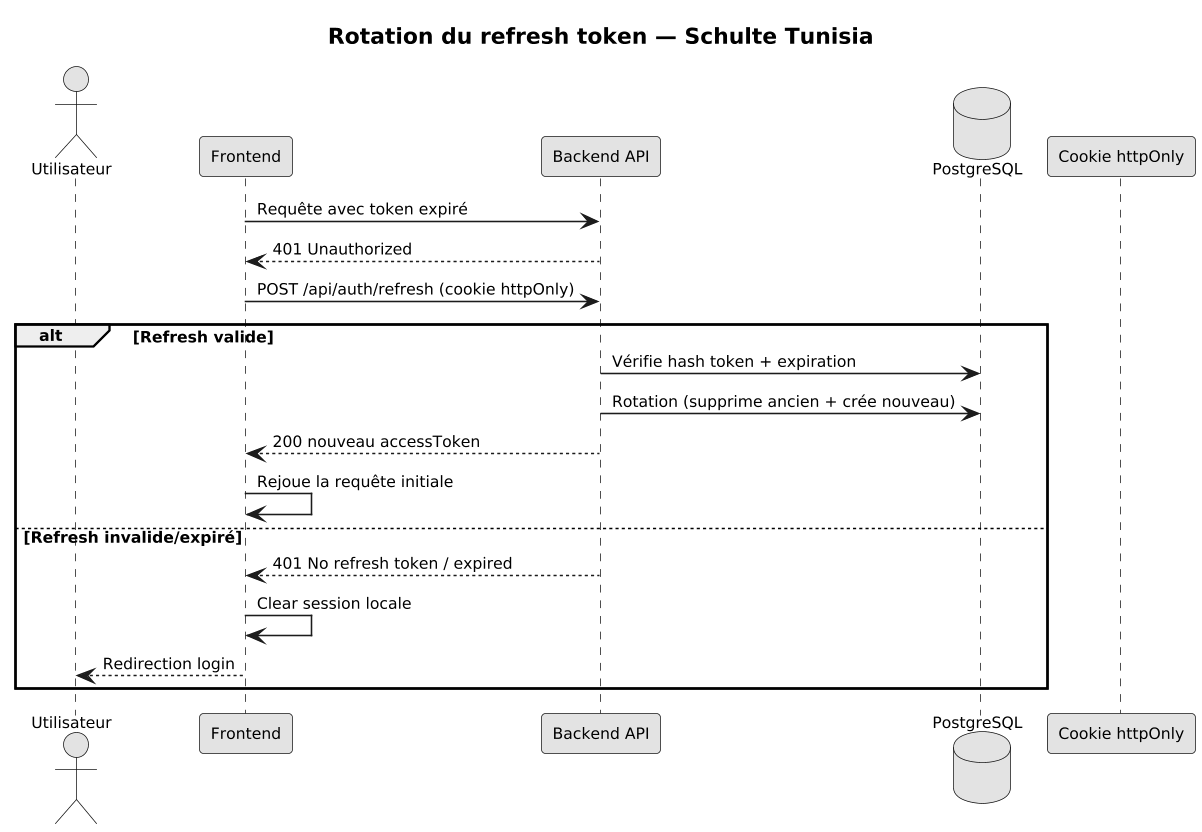
\includegraphics[width=0.90\textwidth]{rotation_refresh_token}
\caption{Rotation des refresh tokens}
\end{figure}

\begin{figure}[H]
\centering
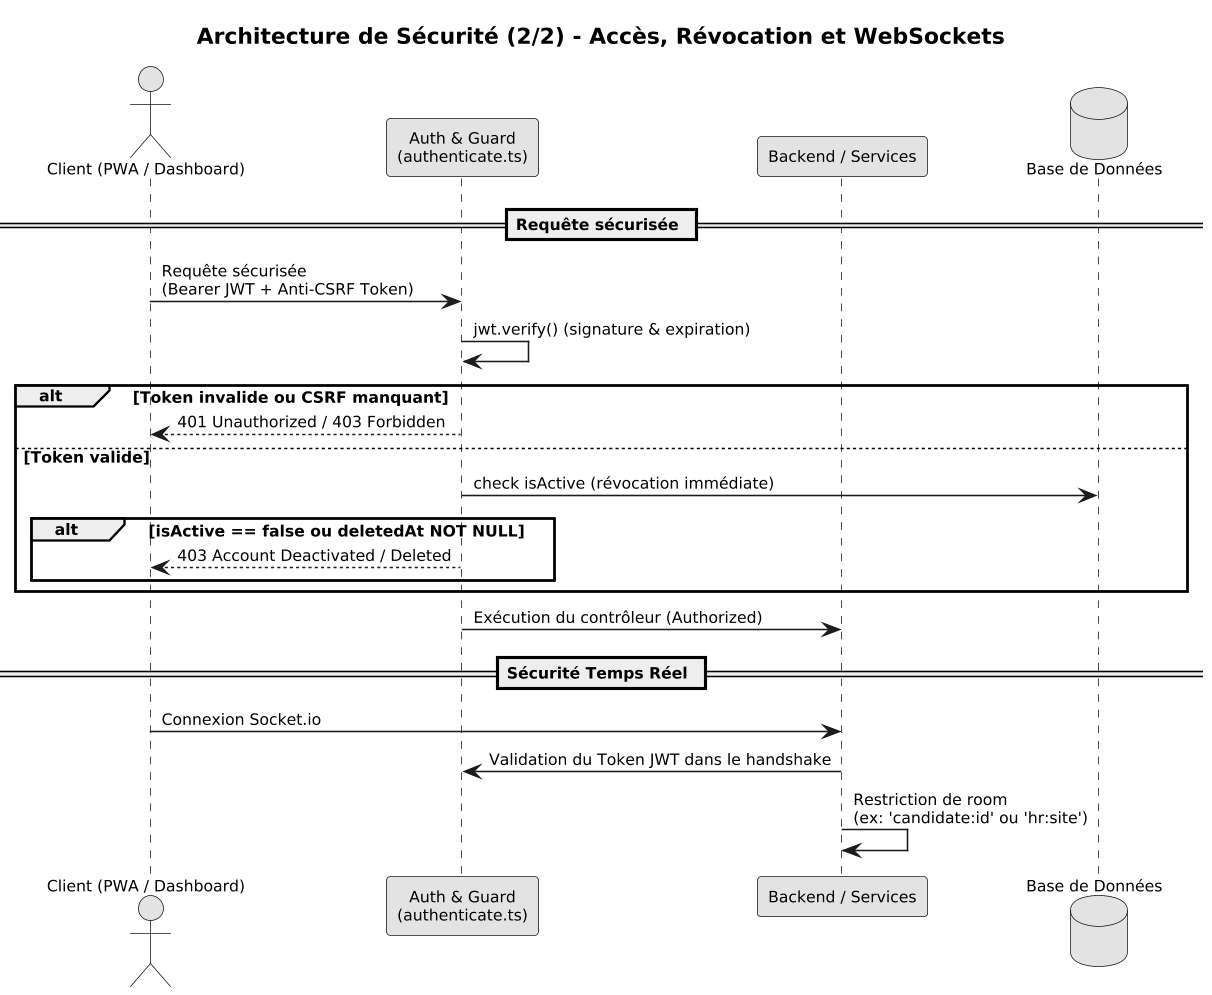
\includegraphics[width=0.90\textwidth]{acces_securise_revocation_websockets}
\caption{Révocation de session et contrôle des accès temps réel}
\end{figure}

\begin{figure}[H]
\centering
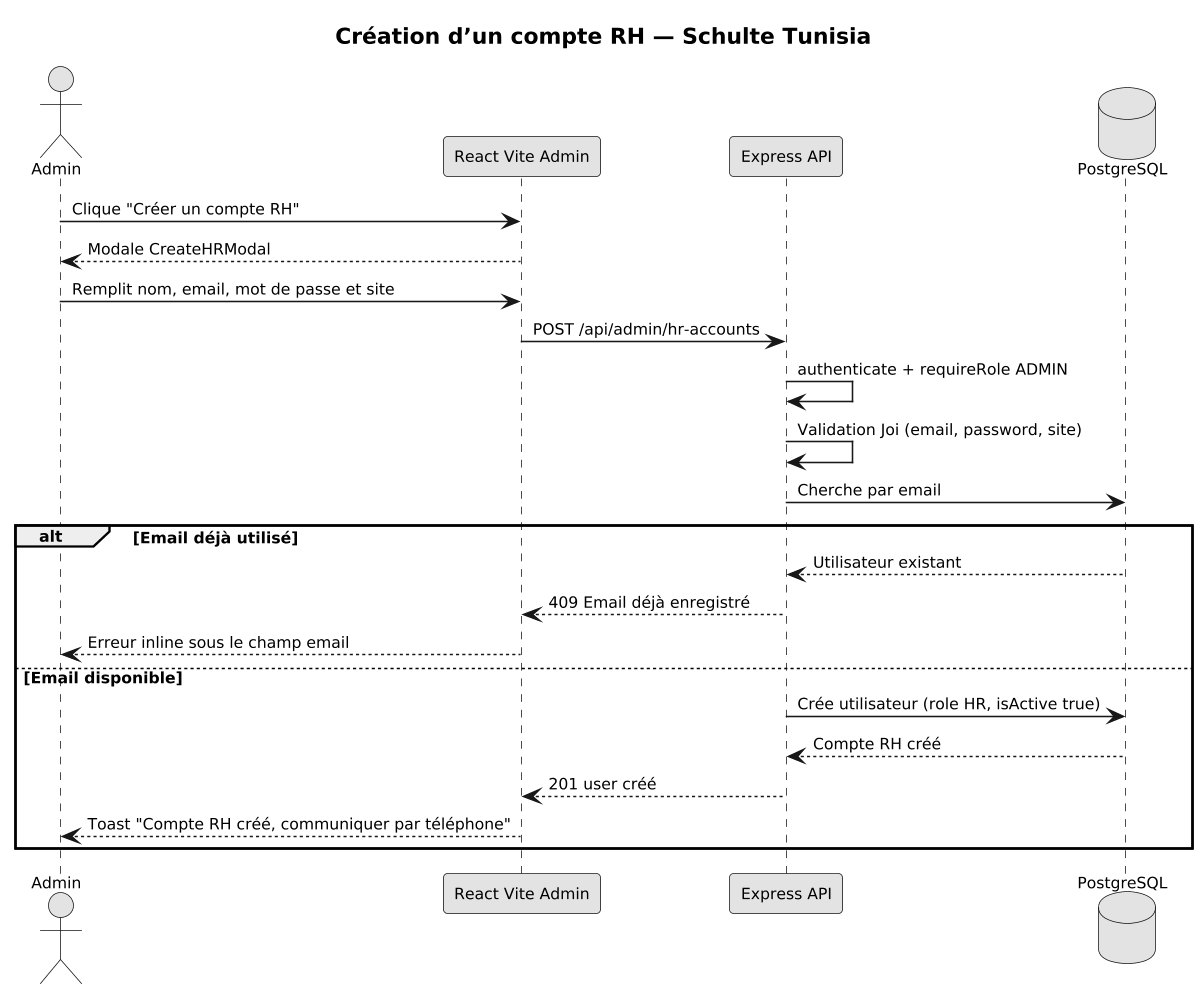
\includegraphics[width=0.90\textwidth]{creation_compte_rh}
\caption{Conception de la création d'un compte RH}
\end{figure}

\begin{figure}[H]
\centering
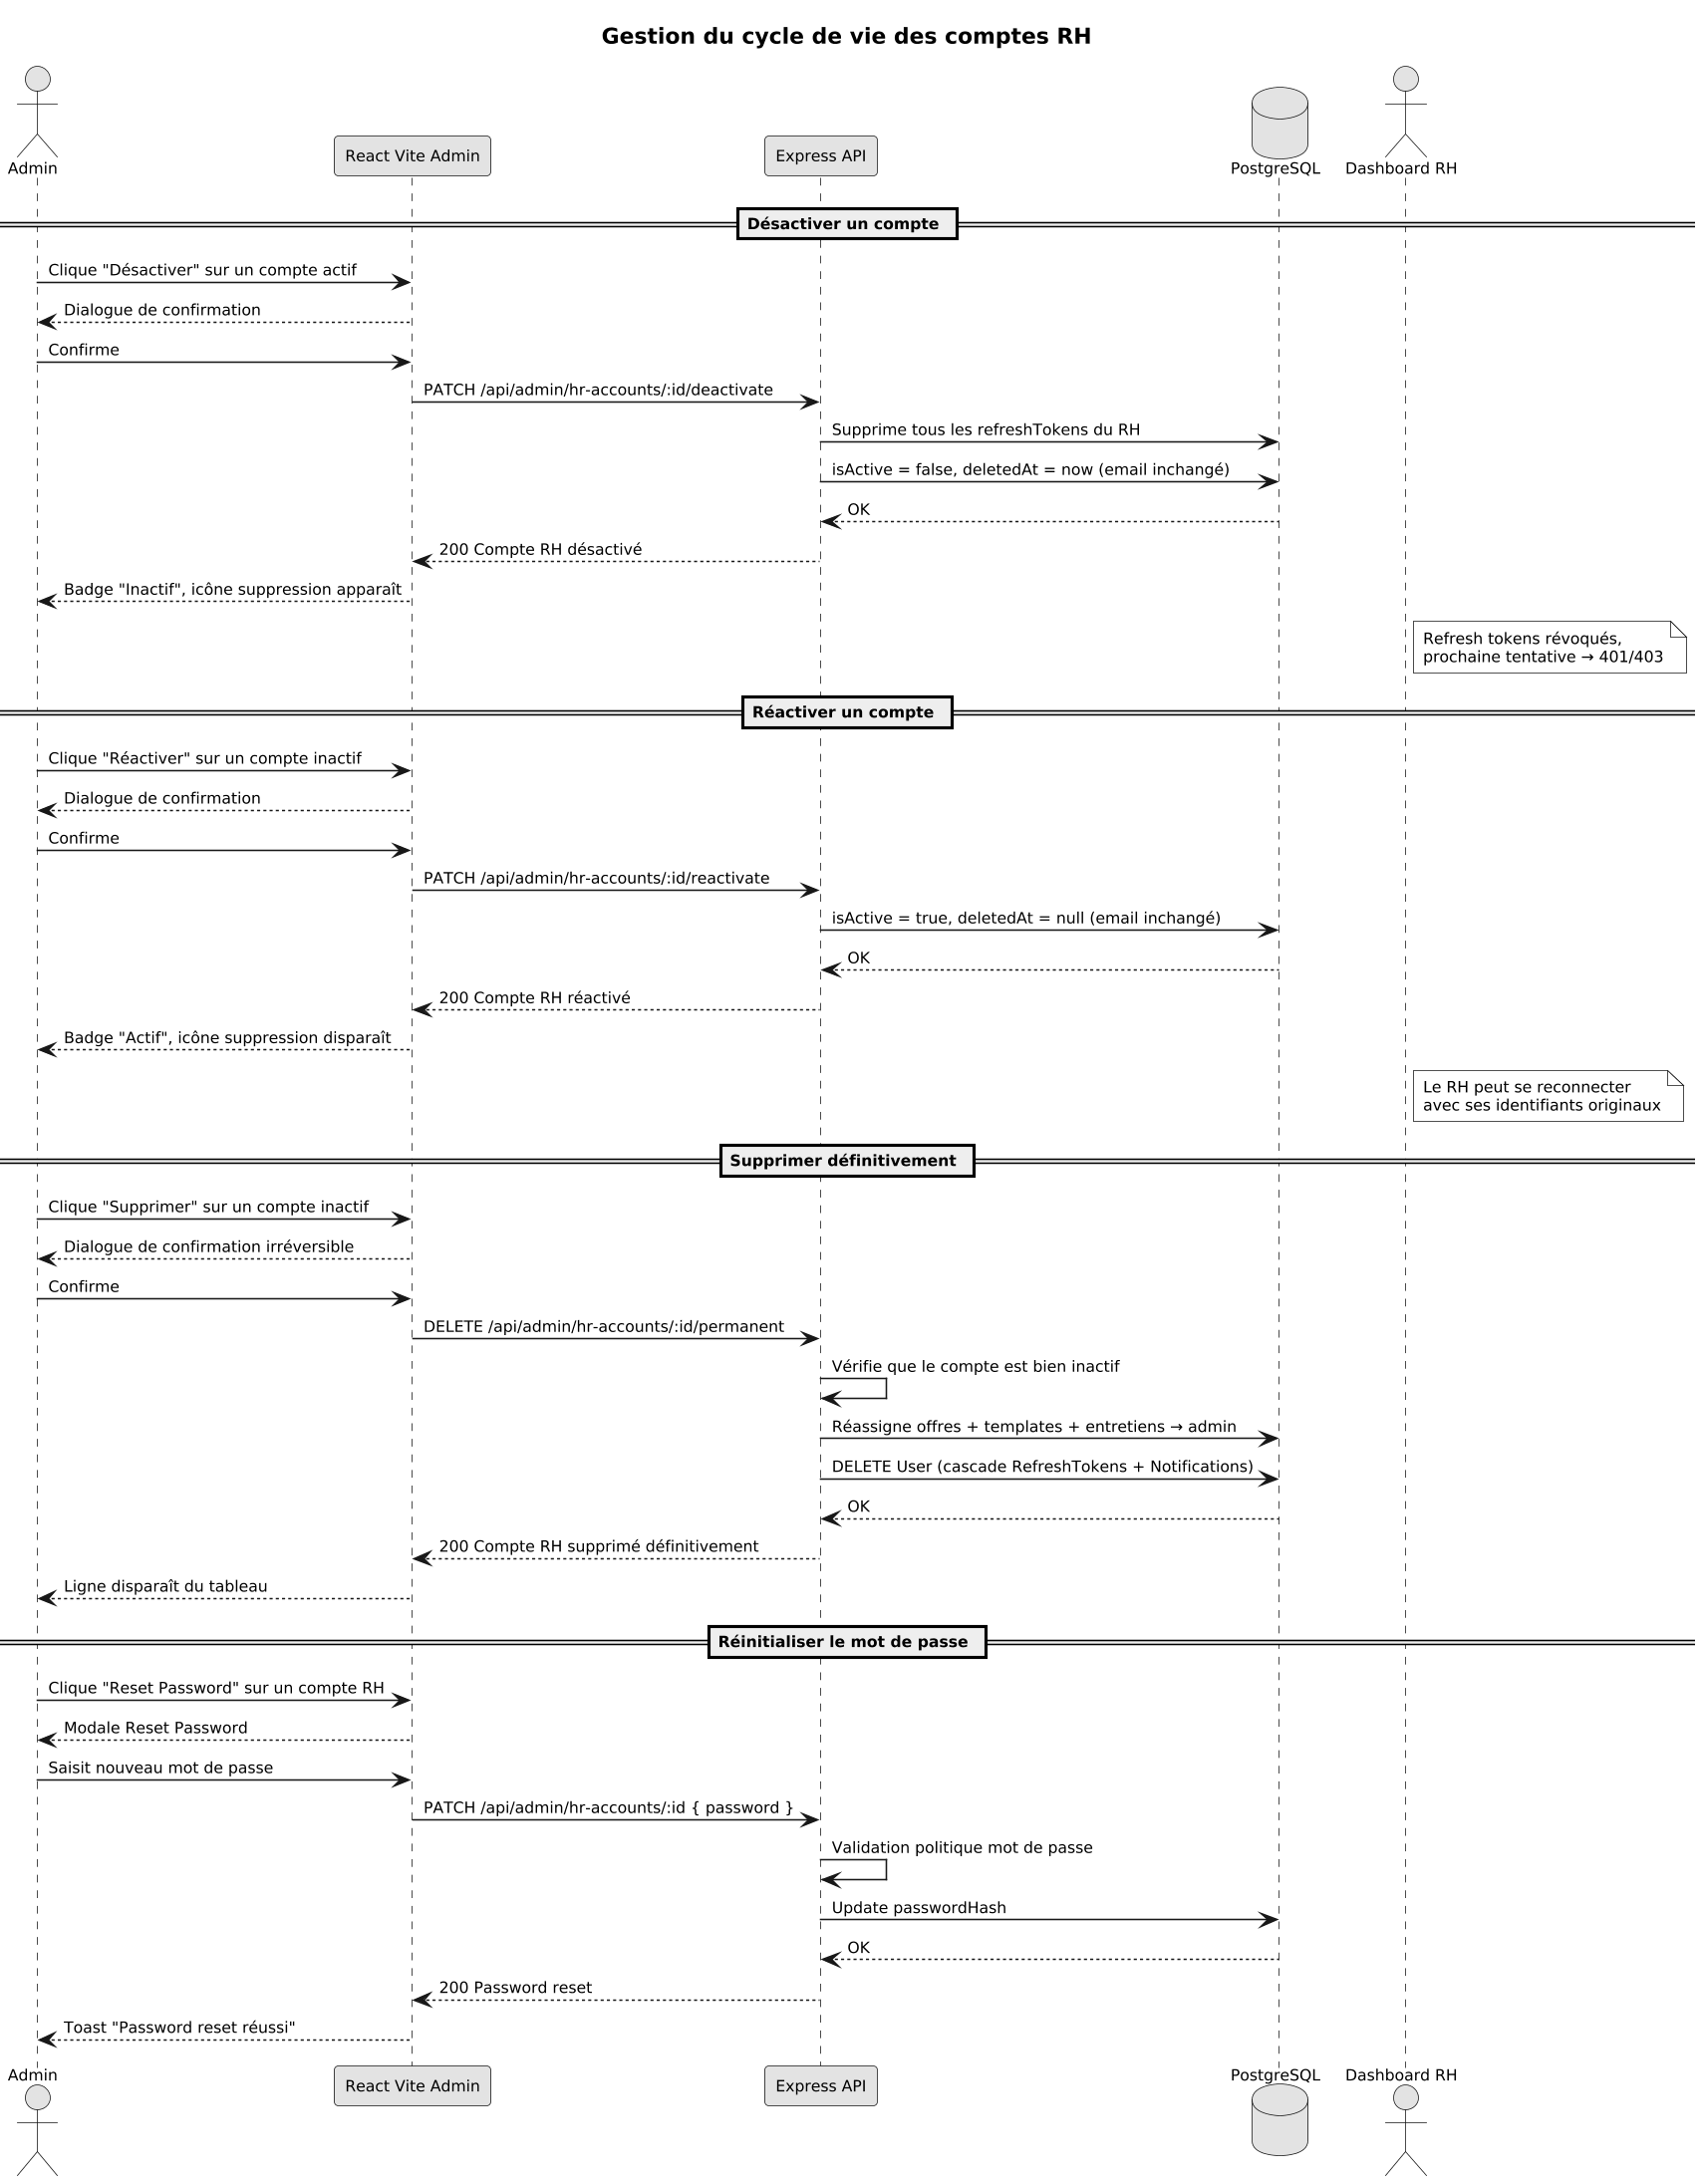
\includegraphics[width=0.90\textwidth]{cycle_vie_compte_rh}
\caption{Cycle de vie d'un compte RH}
\end{figure}

\subsection{Implémentation}

L'implémentation de cette release a renforcé la robustesse backend :
validations strictes, erreurs métier explicites, protections d'accès,
notifications persistantes et automatisations planifiées.

Le résultat est un socle d'exploitation fiable, capable de gérer des cas
réels (sessions à révoquer, comptes à désactiver, statuts à protéger)
sans compromettre la traçabilité du processus.

\subsection{Interfaces}

Les interfaces de gouvernance et de sécurité illustrent la stabilisation
de la plateforme dans des conditions d'usage réel.

\begin{figure}[H]
\centering
\includegraphics[width=0.90\textwidth]{admin_rh_login.png}
\caption{Authentification sécurisée de l'espace RH}
\end{figure}

\begin{figure}[H]
\centering
\includegraphics[width=0.90\textwidth]{admin_comptes_rh.jpg}
\caption{Gestion des comptes RH et contrôle de l'accès}
\end{figure}

% ── Conclusion du chapitre ──────────────────────────────────────
\section*{Conclusion du chapitre 4}
\addcontentsline{toc}{section}{Conclusion du chapitre 4}

Ce chapitre a présenté la conception et la réalisation de la solution selon
un enchaînement progressif par releases Scrum.

La release 1 a livré le flux métier de base, la release 2 a enrichi la
valeur fonctionnelle, et la release 3 a sécurisé puis stabilisé
l'exploitation. Cette progression relie chaque décision de conception à
un usage réel dans l'application.
